\documentclass[10pt, letterpaper, titlepage]{article}

%Size of section header
\usepackage{sectsty}
\sectionfont{\fontsize{12}{15}\selectfont}

%quattrocento font
\usepackage[sfdefault]{quattrocento}

\usepackage{amsmath}
\usepackage{amssymb}
\usepackage{xcolor}
\definecolor{light-gray}{gray}{0.50}%Using light gray instead of red for black and white printers
\usepackage{multicol}

%Fitch-style proofs
\usepackage{lplfitch}
\setlength{\fitchprfwidth}{5.6cm}
\setlength{\fitchctxwidth}{6.1cm}
\newcommand*\lx[1]{{\bf X:} #1}
\newcommand*\lip[1]{{\bf IP:} #1}

%For Modal Logic diagrams
%Setup from:
%http://www.actual.world/resources/tex/doc/TikZ.pdf
\usepackage{tikz}
\usetikzlibrary{positioning,arrows,calc}
\tikzset{modal/.style={>=stealth',shorten >=1pt,shorten <=1pt,auto,node distance=1.5cm,semithick},
    world/.style={circle,draw,minimum size=0.5cm},
    point/.style={circle,draw,inner sep=0.5mm,fill=black},
    reflexive above/.style={->,loop,looseness=9,in=130,out=50},
    reflexive below/.style={->,loop,looseness=7,in=240,out=300},
    reflexive left/.style={->,loop,looseness=7,in=150,out=210},
    reflexive right/.style={->,loop,looseness=7,in=30,out=330}}

% For all metavariables
\usepackage[cal=boondoxo]{mathalfa}
\newcommand*{\meta}[1]{\ensuremath{\mathcal{#1}}}

%DEBUG
%\hbox too wide errors same as assignment 3
%lplfitch doesnt like nested proofs

%Header
\usepackage[margin=1in]{geometry}
\usepackage{fancyhdr}
\setlength{\headheight}{12pt}
\pagestyle{fancy}
\lhead{}
\rhead{UCID: 30063828}

%Change lable to letter from number
\renewcommand{\thesubsection}{\alph{subsection}}

%Title page
\title{PHIL 377 Final}
\author{Instructor: Gillman Glyn Payette
    \\UCID: 30063828}
\date{Summer 2019}

\newcommand{\uline}{\rule{10mm}{0.2mm}}
\newcommand{\Godel}{Gödel }

\begin{document}
    \maketitle
    %P1
    \section{For each item below, provide a Fitch-style proof of the claim.}
        \begin{multicols}{2}
            \subsection{$\vdash \lall x \lall y (x = y \liff y = x)$}
                \fitchctx{
                    \subproof{
                        \pline[1. ]{a = b}
                    }{
                        \pline[2. ]{a = a}[\eqe{1}{1}]\\
                        \pline[3. ]{b = a}[\eqe{1}{2}]
                    }
                    \subproof{
                        \pline[4. ]{b = a}
                    }{
                        \pline[5. ]{b = b}[\eqe{4}{4}]\\
                        \pline[6. ]{a = b}[\eqe{4}{5}]
                    }
                    \pline[7. ]{a = b \liff b = a}[\liffi{1--3}{4--6}]\\
                    \pline[8. ]{\lall y (a = y \liff y = a)}[\lalli{7}]\\
                    \pline[9. ]{\lall x \lall y (x = y \liff y = x)}[\lalli{8}]
                }
    
            \subsection{$\lall x \lall y \lnot x = y 
                \vdash K(a) \land\lnot K(b)$}
                \fitchprf{
                    \pline[1. ]{\lall x \lall y \lnot x = y}
                }{
                    \pline[2. ]{\lall y \lnot a = y}[\lalle{1}]\\
                    \pline[3. ]{\lnot a = a}[\lalle{2}]\\
                    \pline[4. ]{a = a}[\eqi]\\
                    \pline[5. ]{\lfalse}[\lnote{3}, 4]\\
                    \pline[6. ]{K(a) \land \lnot K(b)}[\lx{5}]
                }
        \end{multicols}
            
        \subsection{$\lis y \lnot K(y)
            , \lall x (\lnot A(x) \lif K(x))
            \vdash \lis w (A(w) \lor \lnot L(w,a))$}
            \begin{center}
                \fitchprf{
                    \pline[1. ]{\lis y \lnot K(y)}\\
                    \pline[2. ]{\lall x (\lnot A(x) \lif K(x))}
                }{
                    \pline[3. ]{\lnot A(b) \lif K(b)}[\lalle{2}]\\
                    \subproof{
                        \pline[4. ]{\lnot K(b)}
                    }{
                        \subproof{
                            \pline[5. ]{\lnot A(b)}
                        }{
                            \pline[6. ]{K(b)}[\life{3}{5}]\\
                            \pline[7. ]{\lfalse}[\lnote{4}, 6]
                        }
                        \pline[8. ]{A(b)}[\lip{5--7}]\\
                        \pline[9. ]{A(b) \lor L(b, a)}[\lori{8}]\\
                        \pline[10. ]{\lis w (A(w) \lor L(w, a))}[\lexii{9}]
                    }
                    \pline[11. ]{\lis w (A(w) \lor L(w, a))}[\lexie{1}{4--10}]
                }
            \end{center}
            
        \subsection{$[\lnot L(c,i,b) \lor \lnot(H(c) \lor H(c))]
            , \lall x \lall y (G(x, y) \lif H(c))
            , \lis x G(i, x) \land \lall x \lall y \lall z L(x,y,z)
            \vdash \lfalse$}
            \begin{center}
                \fitchprf{
                    \pline[1. ]{\lnot L(c,i,b) \lor \lnot(H(c) \lor H(c))}\\
                    \pline[2. ]{\lall x \lall y (G(x, y) \lif H(c))}\\
                    \pline[3. ]{\lis x G(i, x) \land \lall x \lall y \lall z L(x,y,z)}
                }{
                    \pline[4. ]{\lall x \lall y \lall z L(x,y,z)}[\lande{3}]\\
                    \pline[5. ]{\lall y \lall z L(c,y,z)}[\lalle{4}]\\
                    \pline[6. ]{\lall z L(c,i,z)}[\lalle{5}]\\
                    \pline[7. ]{L(c,i,b)}[\lalle{6}]\\
                    \subproof{
                        \pline[8. ]{\lnot L(c,i,b)}
                    }{
                        \pline[9. ]{\lfalse}[\lnote{7}, 8]
                    }
                    \pline[10. ]{\lall y (G(i, y) \lif H(c))}[\lalle{2}]\\
                    \pline[11. ]{G(i, j) \lif H(c)}[\lalle{10}]\\
                    \pline[12. ]{\lis x G(i, x)}[\lande{3}]\\
                    \subproof{
                        \pline[13. ]{G(i,j)}
                    }{
                        \pline[14. ]{H(c)}[\life{11}{13}]
                    }
                    \pline[15. ]{H(c)}[\lexie{12}{13--14}]\\
                    \pline[16. ]{H(c) \lor H(c)}[\lori{15}]\\
                    \subproof{
                        \pline[17. ]{\lnot (H(c) \lor H(c))}
                    }{
                        \pline[18. ]{\lfalse}[\lnote{16}, 17]
                    }
                    \pline[19. ]{\lfalse}[\lore{1}{8--9}{17--18}]
                }
            \end{center}
            
    \newpage
    %P2
    \section[]{Some philosophers are travelling to a conference together. Among them are Fitch,
        \Godel, and Hobbes. Consider the following dictionary and domain:
        \begin{itemize}
            \item Domain: The six philosophers going to the conference.
            \item $D(x,y) \uline x$ is driving $\uline y$
            \item $A(x) \uline x$ is in car $A$
            \item $B(x) \uline x$ is in car $B$
            \item $f:$ Fitch; $g:$ \Godel; $h:$ Hobbes
        \end{itemize}
        Using first order logic, formalize the scenarios described in a-d below.
    }
    (Note: Assume 2a is always the case.)
    \subsection{Everyone is in exactly one of the two cars.\\
        (Each person is in at least one of car A or car B, and no one is in both cars.)}
        $\lall x [(A(x) \lor B(x))
            \land \lnot (A(x) \land B(x))]$
    
    \subsection{Drivers are driving everyone in their car.\\
        (A driver drives all of those who happen to be in the car they are driving.)}
        (Note: The clearer version implies theres exists a driver.)\\
        \(
            \lall x \lall y \lis z 
            [
                (
                    D(x, z) \land
                    [
                        (A(x) \land A(y))
                        \lor
                        (B(x) \land B(y))
                    ]
                )
                \lif
                D(x, y)
            ]
            \land
            \lis x \lis y
            D(x,y)
        \)

    \subsection{Either Fitch or \Godel is driving Hobbes.}
        $D(f, h) \lor D(g,h)$

    \subsection{Fitch is travelling with only two of the others.}
        (Note: 'travelling with' means 'being in the same car as'.)\\
        (Note 2: 'only' is defined as an adverb as 'no more than' by https://www.dictionary.com/.)\\
        (Note 3: 'only' is listed as a synonym of 'at most' by https://www.thesaurus.com/.)\\
        (Note 4: The following formula is not concise, but it's algorithmic and simple.)\\
        \(
            \lis x_0 \lis x_1 \lis x_2 \lis x_3 \lis x_4 
            [
                [(((((((((A(f) \land A( x_0 )) \land A( x_1 )) \land\lnot A( x_2 )) \land\lnot A( x_3 )) \land\lnot A( x_4 ))
                        \lor (((((B(f) \land B( x_0 )) \land B( x_1 )) \land\lnot B( x_2 )) \land\lnot B( x_3 )) \land\lnot B( x_4 )))
                            \lor (((((A(f) \land A( x_0 )) \land\lnot A( x_1 )) \land\lnot A( x_2 )) \land\lnot A( x_3 )) \land\lnot A( x_4 )))
                                \lor (((((B(f) \land B( x_0 )) \land\lnot B( x_1 )) \land\lnot B( x_2 )) \land\lnot B( x_3 )) \land\lnot B( x_4 )))
                                    \lor (((((A(f) \land\lnot A( x_0 )) \land\lnot A( x_1 )) \land\lnot A( x_2 )) \land\lnot A( x_3 )) \land\lnot A( x_4 )))
                                        \lor (((((B(f) \land\lnot B( x_0 )) \land\lnot B( x_1 )) \land\lnot B( x_2 )) \land\lnot B( x_3 )) \land\lnot B( x_4 ))]
                \land
                [(((((((((((((\lnot f = x_0 
                    \land\lnot f = x_1 )
                        \land\lnot f = x_2 )
                            \land\lnot f = x_3 )
                                \land\lnot f = x_4 )
                                    \land\lnot x_0 = x_1 )
                                        \land\lnot x_0 = x_2 )
                                            \land\lnot x_0 = x_3 )
                                                \land\lnot x_0 = x_4 )
                                                    \land\lnot x_1 = x_2 )
                                                        \land\lnot x_1 = x_3 )
                                                            \land\lnot x_1 = x_4 )
                                                                \land\lnot x_2 = x_3 )
                                                                    \land\lnot x_2 = x_4 )
                                                                        \land\lnot x_3 = x_4 ]
            ]
        \)

    \newpage
    %P3
    \section{For each of the following modal arguments provide a model that is a counterexample.
        Diagrams that indicate which formulas are true and which are false at which worlds
        is fine. No need for further explanation, if you use a diagram. If you do not use a
        diagram, please provide some explanation of which formulas are true at which worlds.
    }
        The counterexamples for all of the following is world 0. 
        %{\color{red} Gray} text is explanations. 
        {\color{red} Red} text is explanations. 
        \subsection{$\square A \land \lozenge B \vDash_T \square(A \land B)$}
            \begin{center}
                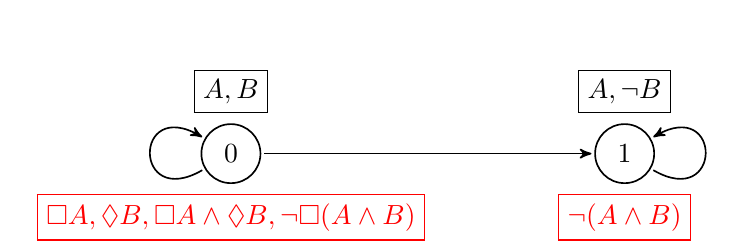
\begin{tikzpicture}[modal, node distance = 5cm, world/.append style={minimum size=.75cm}]
                    \node[world](w0)[
                        label=above:\fbox{$A, B$}
                        , label=below:{\color{red}\fbox{$\square A, \lozenge B, \square A \land \lozenge B, \lnot\square(A \land B)$}}
                        ]{0};
                    \node[world](w1)[
                        label=above:\fbox{$A, \lnot B$}
                        , label=below: {\color{red}\fbox{$\lnot(A \land B)$}}
                        , right of=w0]{1};

                    \path[->] (w0) edge[reflexive left] (w0);
                    \path[->] (w1) edge[reflexive right] (w1);
                    \path[->] (w0) edge (w1);
                \end{tikzpicture}
            \end{center}

        \subsection{$\square A \vDash_T \square\lozenge\square A$}
            \begin{center}
                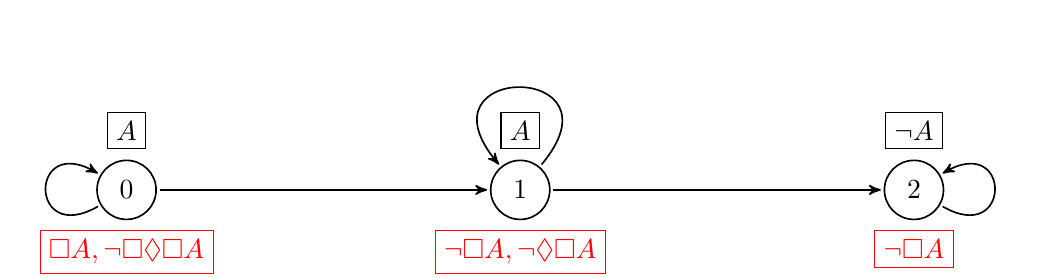
\begin{tikzpicture}[modal, node distance = 5cm, world/.append style={minimum size=.75cm}]
                    \node[world](w0)[
                        label=above:\fbox{$A$}
                        , label=below:{\color{red}\fbox{$\square A, \lnot\square\lozenge\square A$}}]{0};
                    \node[world](w1)[
                        label=above:\fbox{$A$}
                        , label=below:{\color{red}\fbox{$\lnot\square A, \lnot\lozenge\square A$}}
                        , right of=w0]{1};
                    \node[world](w2)[
                        label=above:\fbox{$\lnot A$}
                        , label=below:{\color{red}\fbox{$\lnot\square A$}}
                        , right of=w1]{2};

                    \path[->] (w0) edge[reflexive left] (w0);
                    \path[->] (w1) edge[reflexive above] (w1);
                    \path[->] (w2) edge[reflexive right] (w2);
                    \path[->] (w0) edge (w1);
                    \path[->] (w1) edge (w2);
                \end{tikzpicture}
            \end{center}

        \subsection{$\vDash_{S4} \lozenge\square A \lif \square\lozenge A$}
            \begin{center}
                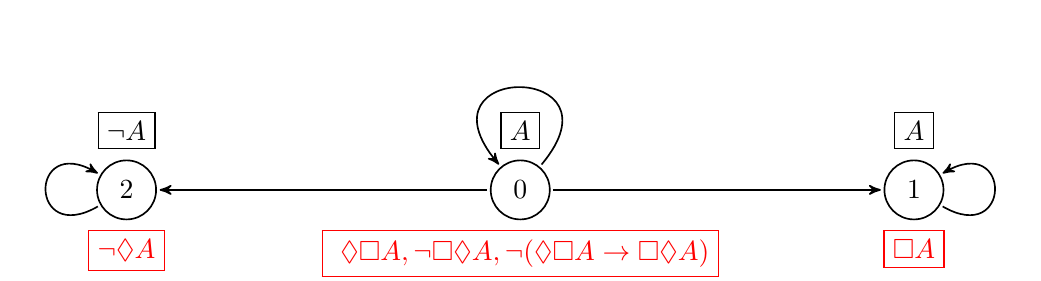
\begin{tikzpicture}[modal, node distance = 5cm, world/.append style={minimum size=.75cm}]
                    \node[world](w0)[
                        label=above:\fbox{$A$}
                        , label=below:{\color{red}\fbox{
                            $\lozenge\square A, \lnot\square\lozenge A
                            , \lnot(\lozenge\square A \lif \square\lozenge A)$}}
                        ]{0};
                    \node[world](w1)[
                        label=above:\fbox{$A$}
                        , label=below:{\color{red}\fbox{$\square A$}}
                        , right of=w0]{1};
                    \node[world](w2)[
                        label=above:\fbox{$\lnot A$}
                        , label=below:{\color{red}\fbox{$\lnot\lozenge A$}}
                        , left of=w0]{2};

                    \path[->] (w0) edge[reflexive above] (w0);
                    \path[->] (w1) edge[reflexive right] (w1);
                    \path[->] (w2) edge[reflexive left] (w2);
                    \path[->] (w0) edge (w1);
                    \path[->] (w0) edge (w2);
                \end{tikzpicture}
            \end{center}

        \subsection{$\square A \lif \lozenge A \vDash_{K4} \lozenge A \lif \square A$}
            \begin{center}
                \begin{tikzpicture}[modal, node distance = 5cm, world/.append style={minimum size=.75cm}]
                    \node[world](w0)[
                        label=above:\fbox{$A$}
                        , label=below:{\color{red}\fbox{
                            $\lnot\square A, \square A \lif \lozenge A
                            , \lozenge A, \lnot(\lozenge A \lif \square A)$}}]{0};
                    \node[world](w1)[
                        label=above:\fbox{$\lnot A$}
                        , right of=w1]{1};

                    \path[->] (w0) edge[reflexive above] (w0);
                    \path[->] (w0) edge (w1);
                \end{tikzpicture}
            \end{center}
\end{document}
